\task{Через тернии к звёздам}
\begin{enumerate}

\item Рассмотрим вершины правильного $n$--угольника. Расстоянием $d\,(A,B)$ между двумя вершинами будем называть длину кратчайшего пути между ними по сторонам $n$--угольника (см.\,рис.\,S1). Докажите, что для любых трёх вершин $A$, $B$, $C$ выполнено неравенство $d\,(A,B) + d\,(B,C) \geq d\,(A,C)$.

\item Для данного $n$--угольника, сколько различных значений принимает расстояние между его вершинами? Для данной вершины, сколько других вершин $n$--угольника находятся на фиксированном расстоянии от неё? Сколько вершин $n$--угольника наиболее удалены от данной?

\item Обратите внимание на то, что расстояние между вершинами не меняется при вращении $n$--угольника. Попробуйте определить расстояние между вершинами так, чтобы оно менялось при поворотах многоугольника. Правда ли, что любое расстояние, сохраняющееся при вращении, отличается от нашего умножением на какое-то число?

%%%%%%%%%%%%

\vspace{-0.6cm}
\begin{center}
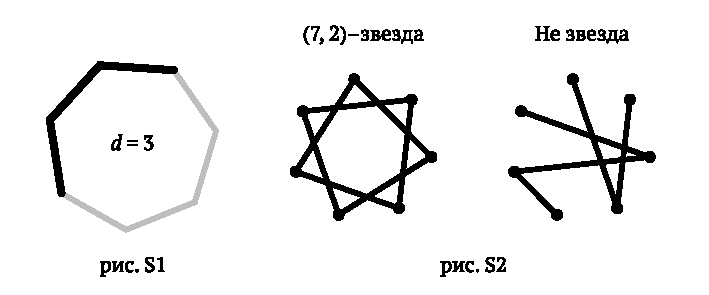
\includegraphics[width=10.5cm]{stats/2017/images/star_defs.pdf}
\end{center} \vspace{-0.7cm}

\item Фиксируем правильный $n$--угольник. Тогда $(n,k)$--звезда — минимальный набор замкнутых ломаных наименьшей длины такой, что любые две вершины $n$--угольника, находящиеся на расстоянии $k$ друг от друга, соединены ребром одной из ломаных набора (см.\,рис.\,S2). Сколько для данного $n$ существует $(n,k)$--звёзд, состоящих из одной ломаной?

\item Для данных $n$ и $k$, из скольки ломаных состоит $(n,k)$--звезда?

\item Для данных $n$ и $\ell$, сколько $(n,k)$--звёзд состоит ровно из $\ell$ ломаных?

\item Через $\varphi(n)$ обозначим количество натуральных чисел, меньших $n$ и взаимно простых с $n$. Используя свои знания о звёздах, докажите формулу

$$\sum\limits_{d \text{ делит } n}\!\!\!\!\!\varphi(d) = n.$$
\end{enumerate}